% !TeX root=../../main.tex

\chapter{حافظه‌ی کوتاه‌مدت بلند (\lr{LSTM})}
\label{appex:lstm}

شبکه‌های \gls{lstm} یا \lr{LSTM} نسخه‌ی تغییریافته‌ای از شبکه‌های عصبی بازگشتی هستند که یادآوری داده‌های گذشته در آن‌ها تسهیل شده است. مشکل گرادیان کاهشی که در شبکه عصبی بازگشتی وجود داشت نیز در این شبکه‌ها حل شده است. شبکه‌های \lr{LSTM} برای مسائل رده‌بندی، پردازش و پیش‌بینی سری‌های زمانی با استفاده از برچسب‌های زمانی مدت‌های نامعلوم مناسب هستند. این شبکه‌ها مدل را با استفاده از انتشار رو به عقب آموزش می‌دهند. 
\begin{figure}[!ht]
	\centerline{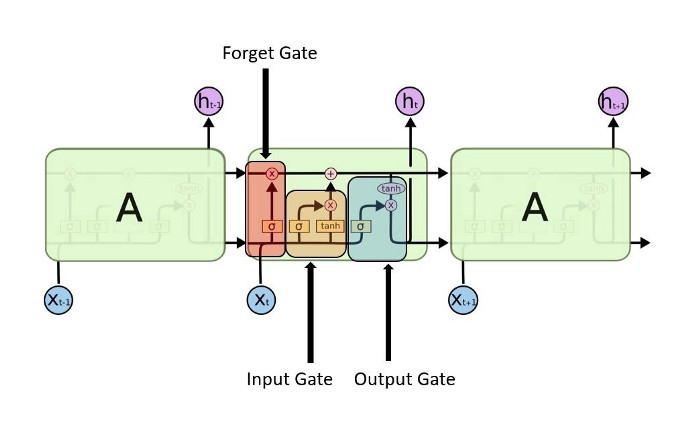
\includegraphics[width=15cm]{chaps/lr/lstm}}
	\caption{ساختار \lr{LSTM}}
	\label{fig:ch_lr:lstm}
\end{figure}
\\
همان‌طور که در شکل \ref{fig:ch_lr:lstm} نمایش داده شده است، در یک شبکه‌ی \lr{LSTM} سه دریچه وجود دارد:

\subsubsection*{دریچه‌های \lr{LSTM}}
\textbf{1) دریچه‌ی ورودی}:
با استفاده از این دریچه می‌توان دریافت کدام مقدار از ورودی را باید برای تغییر حافظه به کار برد. تابع \gls{sigmoid} تصمیم می‌گیرد مقادیر بین $0$ و $1$ اجازه‌ی ورود دارند و تابع $\tanh$ با ضریب‌دهی (بین $-1$ تا $+1$) به مقادیر، در مورد اهمیت آن‌ها تصمیم می‌گیرد.
\begin{equation}
	\begin{aligned}
		i_t &= \sigma (W_i \cdot [h_{t-1}, x_t]+b_i)
		\\
		\tilde{C}_t &= \tanh(W_C \cdot [h_{t-1}, x_t] + b_C)
	\end{aligned}
	\label{eq:ch_lr:lstm_in}
\end{equation}

\textbf{2) دریچه‌ی فراموشی}:
از طریق این دریچه می‌توان جزئیاتی را که باید از بلوک حذف شوند، تشخیص داد. تصمیم‌گیری در این مورد برعهده‌ی تابع \gls{sigmoid} است. این تابع با توجه به حالت قبلی $h_{t-1}$ و ورودی محتوا $X_t$، عددی بین $0$ تا $1$ به هرکدام از اعداد موجود در حالت سلولی $C_{t-1}$ اختصاص می‌دهد؛ $0$ نشان‌دهنده‌ی حذف آن عدد و $1$ به معنی نگه داشتن آن است.
\begin{equation}
	f_t = \sigma(W_f\cdot [h_{t-1}, x_t] + b_f)
	\label{eq:ch_lr:lstm_loss}
\end{equation}

\textbf{3) دریچه‌ی خروجی}:
ورودی و حافظه‌ی بلوک برای تصمیم‌گیری در مورد خروجی مورد استفاده قرار می‌گیرند. تابع سیگموئید تصمیم می‌گیرد مقادیر بین $0$ و $1$ اجازه‌ی ورود دارند و تابع $\tanh$ با ضریب‌دهی (بین $-1$ تا $+1$) به مقادیر و ضرب آن‌ها در خروجی تابع \gls{sigmoid} در مورد اهمیت آن‌ها تصمیم‌گیری می‌کند.
\begin{equation}
	\begin{aligned}
		o_t &= \sigma (W_o \cdot [h_{t-1}, x_t]+b_o)
		\\
		h_t &= o_t \ast \tanh(C_t)
	\end{aligned}
	\label{eq:ch_lr:lstm_out}
\end{equation}

در حقیقت هدف از طراحی شبکه‌های \lr{LSTM}، حل کردن مشکل وابستگی بلندمدت بود. به این نکته مهم توجه کنید که به یاد سپاری اطلاعات برای بازه‌های زمانی بلند مدت، رفتار پیش‌فرض و عادی شبکه‌های \lr{LSTM} است و ساختار آ‌ن‌ها به صورتی است که اطلاعات خیلی دور را به خوبی یاد می‌گیرند که این ویژگی در ساختار آن‌ها نهفته است.

همه شبکه‌های عصبی بازگشتی به شکل دنباله‌ای (زنجیره‌ای) تکرار شونده از ماژول‌های (واحد‌های) شبکه‌های عصبی هستند. در شبکه‌های عصبی بازگشتی استاندارد، این ماژول‌های تکرار شونده ساختار ساده‌ای دارند، برای مثال تنها شامل یک لایه تانژانتِ هایپربولیک ($\tanh$) هستند.

\begin{figure}[!ht]
	\centerline{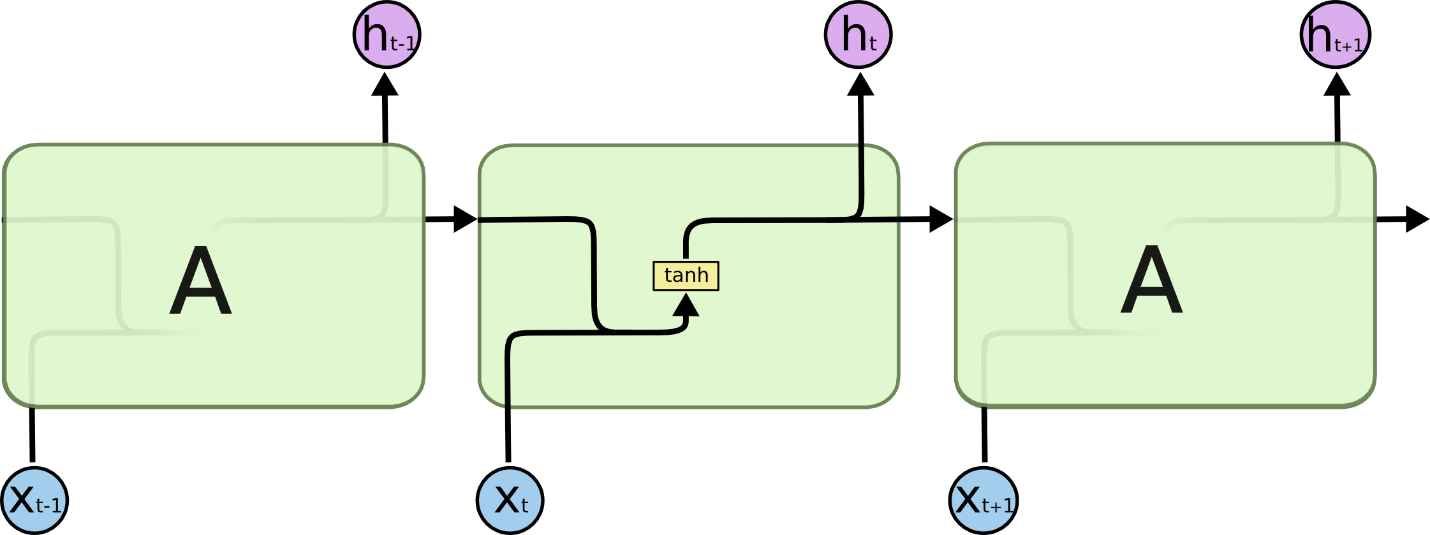
\includegraphics[width=14cm]{chaps/lr/rnn_chain}}
	\caption{
		ماژول‌های تکرار شونده در شبکه‌های عصبی بازگشتی استاندارد فقط دارای یک لایه هستند.
	}
	\label{fig:ch_lr:rnn_chain}
\end{figure}

شبکه‌های \lr{LSTM} نیز چنین ساختار دنباله یا زنجیره‌مانندی دارند ولی ماژولِ تکرار شونده ساختار متفاوتی دارد. به جای داشتن تنها یک لایه شبکه عصبی، 4 لایه دارند که طبق ساختار ویژه‌ای با یکدیگر در تعامل و ارتباط هستند.
\begin{figure}[!ht]
	\centerline{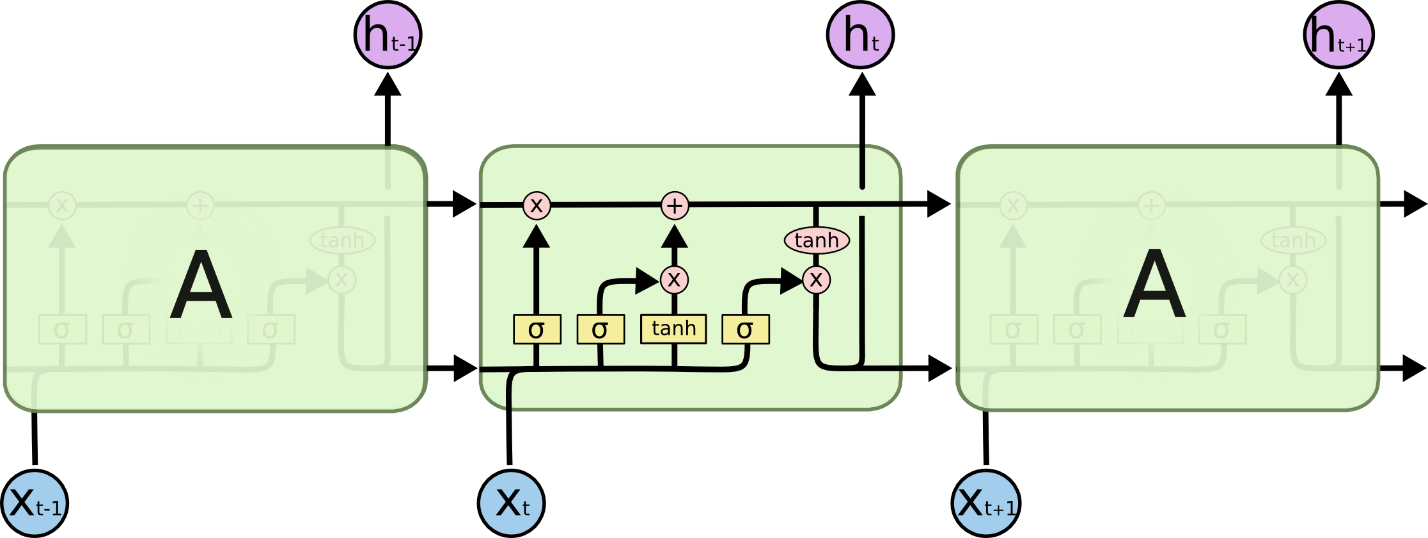
\includegraphics[width=14cm]{chaps/lr/rnn_inside}}
	\caption{
		ماژول‌های تکرار شونده در \lr{LSTM}ها دارای 4 لایه هستند که با هم در تعامل می‌باشند.
	}
	\label{fig:ch_lr:rnn_inside}
\end{figure} 
در ادامه قدم به قدم ساختار شبکه‌های \gls{lstm} را توضیح خواهیم داد. اما در ابتدا معنی هر کدام از شکل‌ و علامت‌هایی را که از آن‌ها استفاده خواهیم کرد توضیح می‌دهیم.
\begin{figure}[!ht]
	\centerline{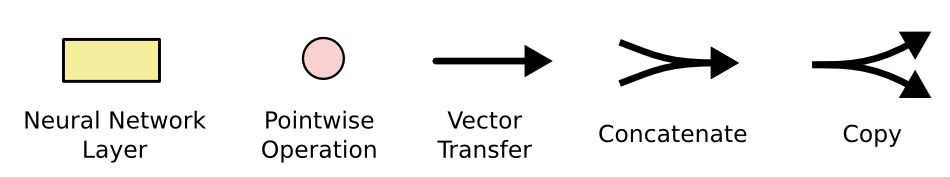
\includegraphics[width=14cm]{chaps/lr/lstm_legend}}
	\caption{
		اشکال از راست به چپ به تریب برابر هستند با: کپی کردن، وصل کردن، بردار انتقال، عملیات نقطه به نقطه، یک لایه‌ی شبکه عصبی.
	}
	\label{fig:ch_lr:lstm_legend}
\end{figure} 
در شکل \ref{fig:ch_lr:lstm_legend}، هر خط یک بردار را به صورت کامل از خروجی یک گره به ورودی گره دیگر انتقال می‌دهد. دایره‌های صورتی نمایش دهنده عملیات‌های نقطه‌ به نقطه مانند «جمع کردن دو بردار» هستند. مستطیل‌های زرد، لایه‌‌های شبکه‌های عصبی هستند که شبکه پارامتر‌های آن‌ها را یاد می‌گیرد. خط‌هایی که با هم ادغام می‌شوند نشان‌دهنده \gls{concatenation} و خط‌هایی که چند شاخه می‌شوند نشان دهنده‌ای این موضوع است که محتوای آن‌ها کپی و به بخش‌های مختلف ارسال می‌شود.
\\
\\
عنصر اصلی \lr{LSTM}ها سلول حالت\LTRfootnote{Cell state} است که در حقیقت یک خط افقی است که در بالای شکل \ref{fig:ch_lr:lstm_cellState1} قرار دارد.
سلول حالت را می‌توان به صورت یک تسمه نقاله تصور کرد که از اول تا آخر دنباله یا همان زنجیره با تعاملات خطیِ جزئی در حرکت است (یعنی ساختار آن بسیار ساده است و تغییرات کمی در آن اتفاق می‌افتد).
\begin{figure}[!ht]
	\centerline{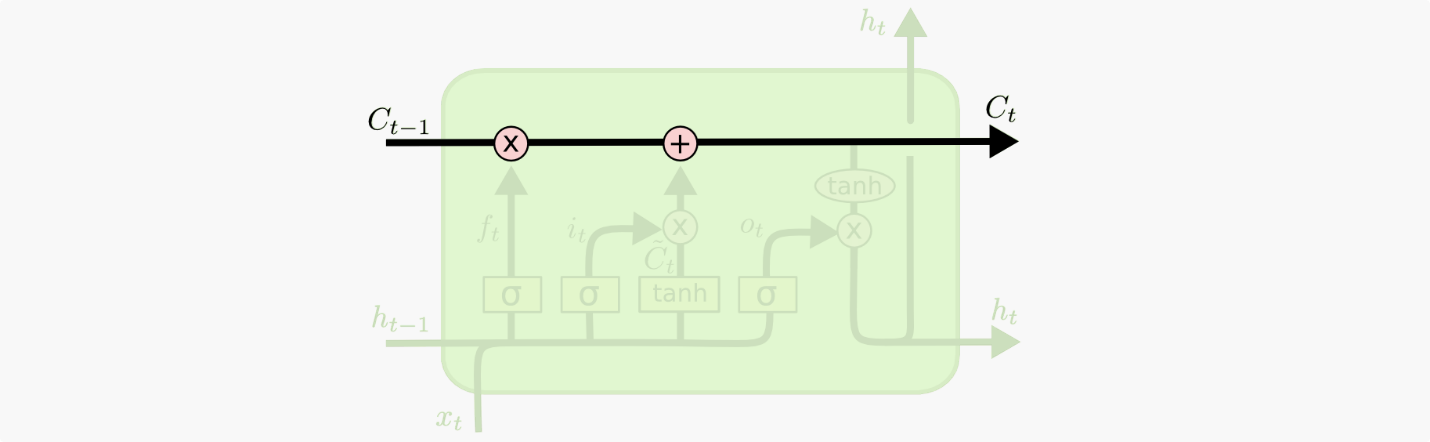
\includegraphics[width=15cm]{chaps/lr/lstm_cellState1}}
	\caption{
		سلول حالت در ماژول \lr{LSTM}
	}
	\label{fig:ch_lr:lstm_cellState1}
\end{figure} 
\\
\lr{LSTM} 
این توانائی را دارد که اطلاعات جدیدی را به سلول حالت اضافه یا اطلاعات آن را حذف کنید. این کار توسط ساختارهای دقیقی به نام \glspl{gate} انجام می‌شود. \glspl{gate}‌ راهی هستند برای ورود اختیاری اطلاعات. آن‌ها از یک لایه شبکه عصبیِ \gls{sigmoid} به همراه یک عملگر ضرب نقطه به نقطه تشکلیل شده‌اند.
\begin{figure}[!ht]
	\centerline{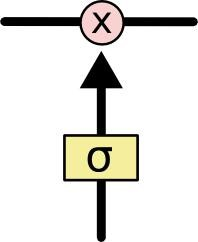
\includegraphics[width=3cm]{chaps/lr/lstm_2}}
	\caption{
		نمایی از نحوه تاثیر و ورود اطلاعات به سلول حالت
	}
	\label{fig:ch_lr:lstm_2}
\end{figure} 
\\
خروجی لایه \gls{sigmoid} عددی بین صفر و یک است، که نشان می‌دهد چه مقدار از وروی باید به خروجی ارسال شود. مقدار صفر یعنی هیچ اطلاعاتی نباید به خروجی ارسال شود در حالی که مقدار یک یعنی تمام ورودی به خروجی ارسال شود!
\\
\\
\lr{LSTM}
دارای 3 \gls{gate} مشابه برای کنترل مقدار سلول حالت است که در ادامه به بررسی قدم به قدمِ آن‌ها از لحظه ورود تا خروج اطلاعات خواهیم پرداخت.
\\
قدم اول در \lr{LSTM} تصمیم در مورد اطلاعاتی است که می‌خواهیم آن‌ها را از سلول حالت پاک کنیم. این تصمیم توسط یک لایه \gls{sigmoid} به نام «دروازه فراموشی\LTRfootnote{Forget gate}» انجام می‌شود. این \gls{gate} با توجه به مقادیر $h_{t-1}$ و $x_t$، برای هر عدد، مقدار صفر یا یک را در سلول حالتِ $C_{t-1}$ به خروجی می‌برد. مقدار یک یعنی به صورت کامل مقدار حال حاضرِ سلول حالت $C_{t-1}$ را به $C_t$ انتقال داده شود و مقدار صفر یعنی به صورت کامل اطلاعات سلول حالت کنونی $C_{t-1}$ را پاک شود و هیچ مقداری از آن  به $C_t$ برده نشود. بیاید به مثال قبلی‌مان که یک مدل زبانی‌ای بود که در آن تلاش داشتیم کلمه بعدی را بر اساس همه کلمه‌های قبلی حدس بزنیم، برگردیم. در چنین مسأله‌ای، سلول حالت ممکن است دربردارنده جنسیت فاعل کنونی باشد، که با توجه به آن می‌توانیم تشخیص دهیم از چه ضمیری باید استفاده کنیم. زمانی که یک فاعل جدید در جمله ظاهر می‌شود، می‌بایست جنسیت فاعل قبلی حذف شود.
\begin{figure}[!ht]
	\centerline{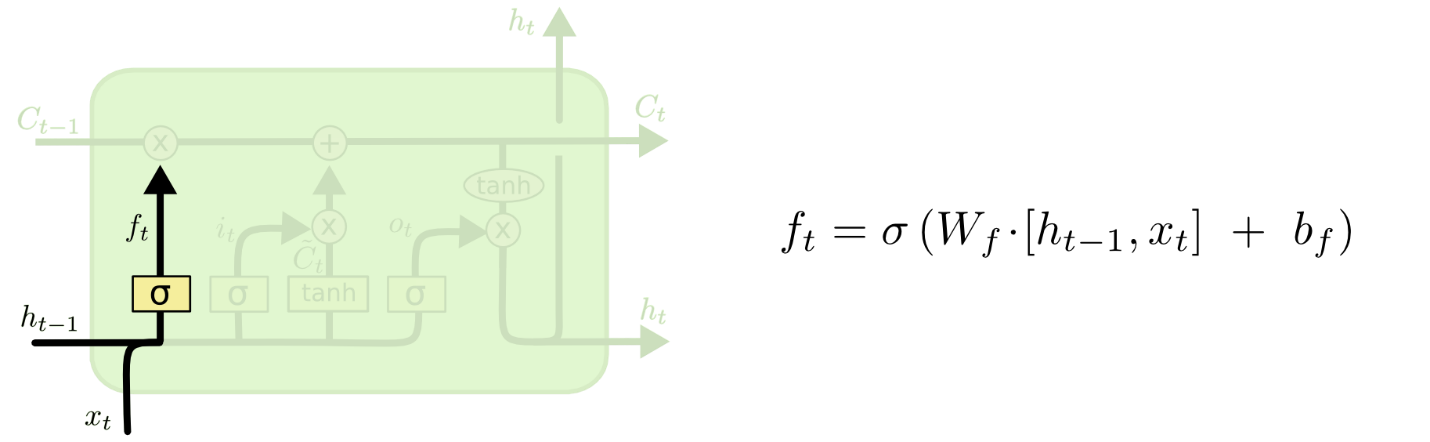
\includegraphics[width=15cm]{chaps/lr/lstm_3}}
	\caption{
		قدم اول در پاک کردن اطلاعات از سلول حالت در وضعیت ورودی
	}
	\label{fig:ch_lr:lstm_3}
\end{figure} 
\\
قدم بعدی این است که تصمیم بگیریم چه اطلاعات جدیدی را می‌خواهیم در سلول حالت ذخیره کنیم. این تصمیم دو بخشی است. ابتدا یک لایه سیگموید به نام دروازه ورودی\LTRfootnote{Input gate} داریم که تصمیم می‌گیرد چه مقادیری به‌روز خواهند شد. مرحله بعدی یک لایه تانژانت هایپربولیک است که برداری از مقادیر به نام $\tilde{C}_t$ می‌سازد که می‌توان آن‌ها را به سلول حالت اضافه کرد. در مرحله بعد، ما این دو مرحله را با هم ترکیب می‌کنیم تا مقدار سلول حالت را به‌روز کنیم.
\\
در مثال مدل زبانی‌ای که پیش‌تر داشتیم، قصد داریم جنسیت فاعل جدید را به سلول حالت اضافه کنیم تا جایگزین جنسیت فاعل قبلی شود که در مرحله قبلی تصمیم گرفتیم آن را فراموش کنیم.
\begin{figure}[!ht]
	\centerline{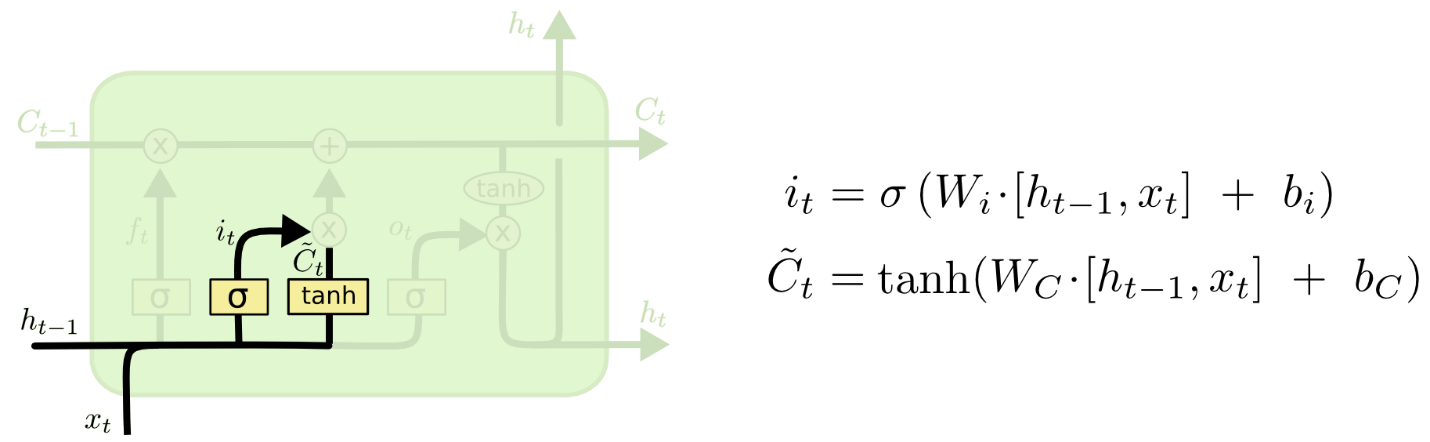
\includegraphics[width=15cm]{chaps/lr/lstm_4}}
	\caption{
		قدم دوم در اضافه کردن اطلاعات جدید به سلول حالت
	}
	\label{fig:ch_lr:lstm_4}
\end{figure} 
\\
حال زمان آن فرا رسیده است که سلول حالت قدیمی یعنی $C_{t-1}$ را سلول حالت جدید یعنی $C_t$ به‌روز کنیم. در مراحل قبلی تصمیم گرفته شد که چه کنیم و در حال حاضر تنها لازم است تصمیماتی را که گرفته شد عملی کنیم.
\\
ما مقدار قبلی سلول حالت را در $f_t$ ضرب می‌کنیم که یعنی فراموش کردن اطلاعاتی که پیش‌تر تصمیم گرفتیم آن‌ها را فراموش کنیم. سپس $i_t \ast \tilde{C}_t$ را به آن اضافه می‌کنیم. در حال حاضر مقادیر جدید سلول حالت با توجه به تصمیماتی که پیش‌تر گرفته شده بود بدست آمده‌اند. در مثال مدل زبانی، اینجا دقیقاً جائی است که اطلاعاتی که در مورد جنسیت قبلی داشتیم را دور می‌ریزیم و اطلاعات جدید را اضافه می‌کنیم.
\begin{figure}[!ht]
	\centerline{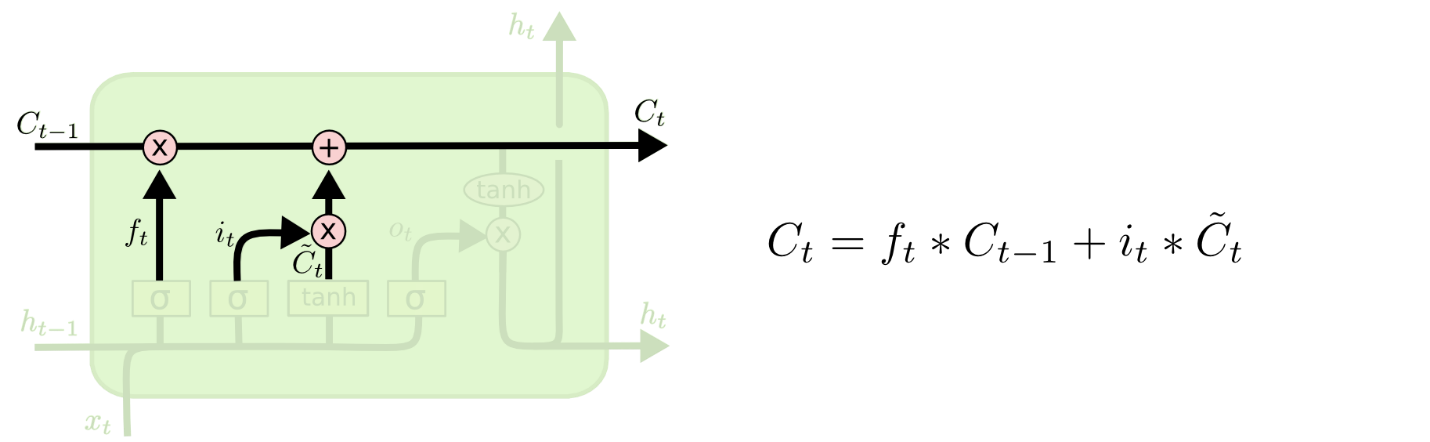
\includegraphics[width=15cm]{chaps/lr/lstm_5}}
	\caption{
		به‌روز رسانی اطلاعات در سلول حالت
	}
	\label{fig:ch_lr:lstm_5}
\end{figure} 
\\
در نهایت باید تصمیم بگیریم قرار است چه اطلاعاتی را به خروجی ببریم. این خروجی با در نظر گرفتن مقدار سلول حالت خواهد بود، ولی از فیلتر مشخصی عبور خواهد کرد. در ابتدا، یک لایه سیگموید داریم که تصمیم می‌گیرد چه بخشی از سلول حالت قرار است به خروجی برده شود. سپس مقدار سلول حالت (پس از به‌روز شدن در مراحل قبلی) را به یک لایه تانژانت هایپربولیک (تا مقادیر بین $-1$ و $+1$ باشند) می‌دهیم و مقدار آن را در خروجی لایه \gls{sigmoid} قبلی ضرب می‌کنیم تا تنها بخش‌هایی که مد نظرمان است به خروجی برود.
\\
در مثال مدل زبانی، با توجه به اینکه تنها فاعل را دیده‌است، در صورتی که بخواهیم کلمه بعدی را حدس بزنیم، ممکن است بخواهد اطلاعاتی در ارتباط با فعل را به خروجی ببرد. برای مثال ممکن است اینکه فاعل مفرد یا جمع است را به خروجی ببرد، که ما با توجه به آن بدانیم فعل به چه فرمی خواهد بود.
\begin{figure}[!ht]
	\centerline{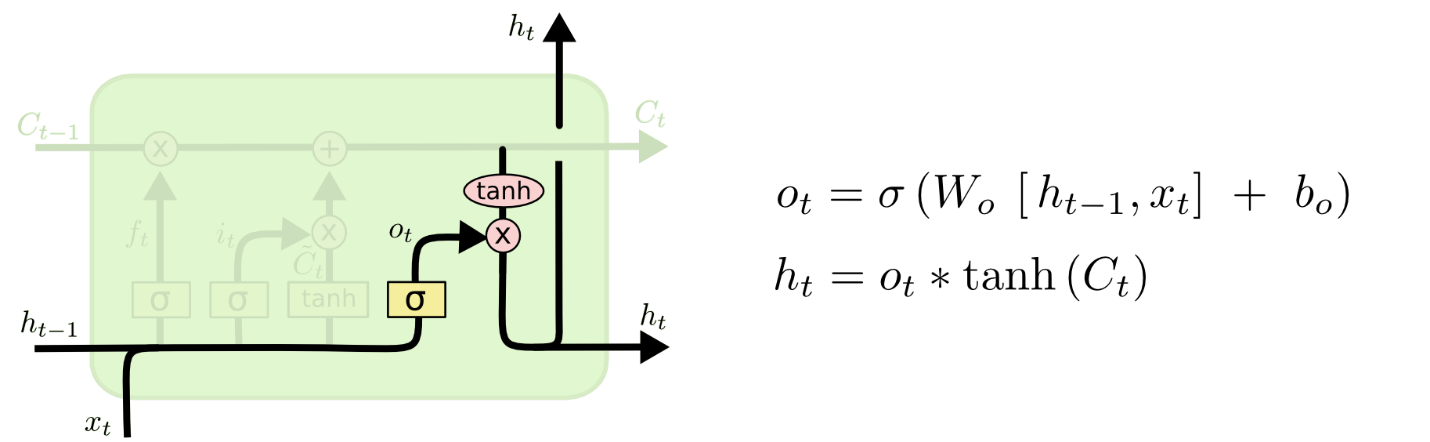
\includegraphics[width=15cm]{chaps/lr/lstm_6}}
	\caption{
		قدم نهایی برای تولید خروجی ماژول \lr{LSTM}
	}
	\label{fig:ch_lr:lstm_6}
\end{figure} 
